\chapter{Siblings in the \fhkb}
\label{chap:sibs}

In this chapter you will:
\begin{enumerate}
\item Explore options for determining finding siblings;
\item Meet some of the limitations in OWL;
\item Choose one of the options explored;
\item Add facts for siblings;
\item Use sub-property chains to find aunts and uncles;
\end{enumerate}

\snapshot{There is a snapshot of the ontology as required at this point in the tutorial available at \fhkbhome.}

%\dragon{For \protege users: It can happen that accessing the individual tab after reasoning causes \protege to crash. Should that be the case, we recommend to rely on the DL query tab as your means of testing the \fhkb ontology and its inferences. Also, as of the time of this writing\footnote{February 2013}, the reasoners Pellet 2.3.0 did not respond reliably towards the end of this chapter. FaCT++ 1.6.2 did well up until the end of chapter~\ref{chap:marriage} (even reasonably fast). HermiT 1.3.6 worked fine until the very end, albeit a bit slowly.}
\section{Blood relations}
\label{sec:br}

Do the following first:
\steps{The bloodrelation object property}{
\item Create an \con{hasBloodrelation} object property, making it a sub-property of hasRelation.
\item Add appropriate property characteristics.
\item Make the already existing \con{hasAncestor} property a sub-property of \con{hasBloodrelation}.
}

Does a blood relation of Robert have the same relationship to Robert (symmetry)? Is a blood relation of Robert's blood relation a blood relation of Robert (transitivity)? Think of an aunt by marriage; her children are my cousins and blood relations via my uncle, but my aunt is not my blood relation. My siblings share parents; male siblings are brothers and female siblings are sisters. So far we have asserted parentage facts for the \person in our ABox. Remember that our parentage properties have inverses, so if we have added an \con{hasFather} property between a \person and a \man, we infer the \con{isFatherOf} property between that \man and that \person. 

\section{Siblings: Option One}
\label{sec:sib1}
We should have enough information within the \fhkb to infer siblings. We could use a sub-property chain such as:
\\\\
\owlcode{
ObjectProperty: hasSibling

SubPropertyOf: hasBloodrelation

Characteristics: Symmetric, transitive

SubPropertyChain: hasParent o isParentOf
}
\\\\
We make a property of \con{hasSibling} and make it a sub-property of \con{hasBloodrelation}. Remember, think of the objects involved and the implications we want to follow; being a sibling implies being a blood relation, it does not imply any of the other relationships we have in the \fhkb. 

Note that we have made \con{hasSibling} symmetric; if Robert is sibling of Richard, then Richard is sibling of Robert. We should also think about transitivity; if David is sibling of Peter and Peter is sibling of John, then David is sibling of John. So, we make \con{hasSibling} symmetric and transitive (see Figure~\ref{fig:sib_trans}).{\herebedragons} However, we must take care of half-siblings: child~1 and child~2 share a mother, but not a father; child~2 and child~3 share the father, but not the mother -- child~1 and child~3 are not even half-siblings. However, at least for the moment, we will simply ignore this inconvenience, largely so that we can explore what happens with different modelling options.

\begin{figure}
\begin{center}
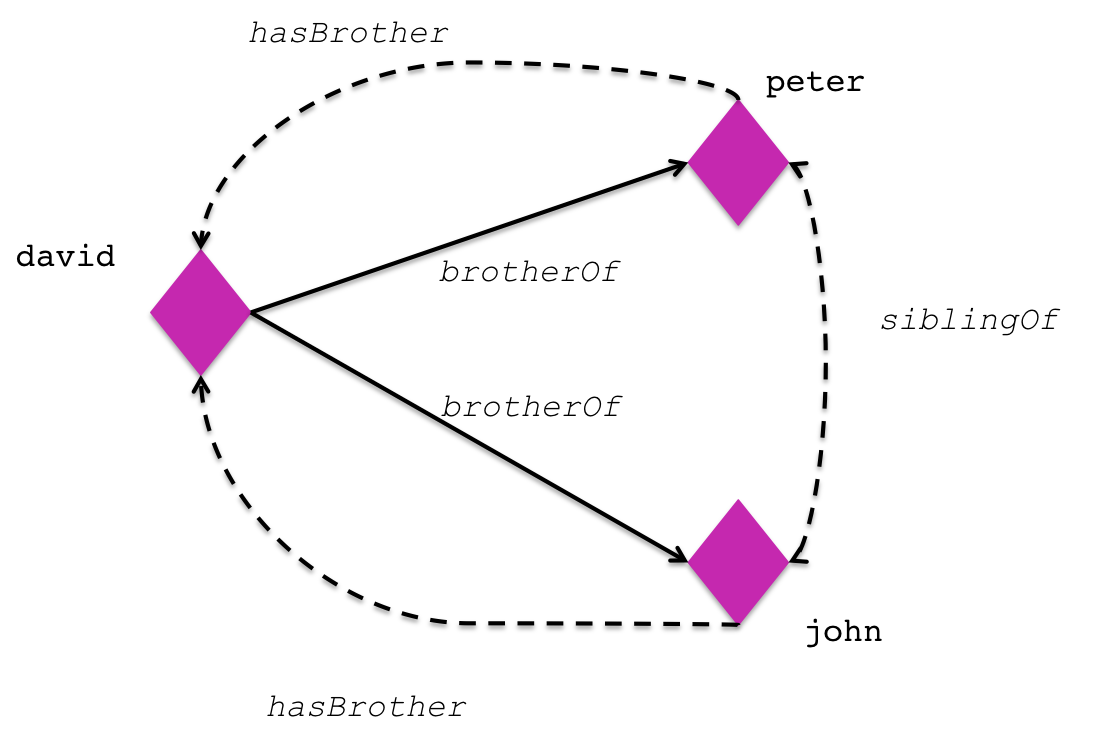
\includegraphics[width=\figwidth]{figures/siblings}\caption{Showing the symmetry and transitivity of the \con{hasSibling} (siblingof) property by looking at the brothers David, John and Peter}\label{fig:sib_trans}
\end{center}
\end{figure}

We also have the implication using three objects (see Figure~\ref{fig:siblings}):
\begin{enumerate}
\item Robert holds a \con{hasParent} property with David;
\item David holds an \con{isFatherOf} property with Richard;
\item This implies that Robert holds a \con{hasSibling} property with Richard;
\item As \con{hasSibling} is symmetric, Richard holds an \con{hasSibling} property with Robert. 
\end{enumerate}

\begin{figure}
\begin{center}
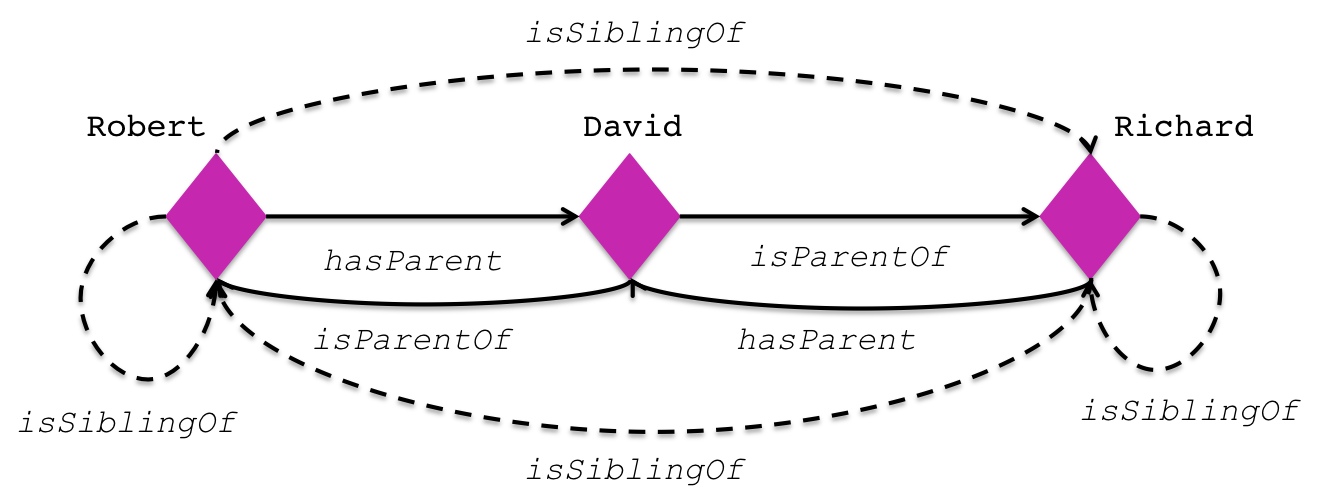
\includegraphics[width=\figwidth]{figures/sibling_path}
\caption{Tracing out the sub-property chain for \con{hasSibling}; note that Robert is a sibling of himself by this path}
\label{fig:siblings}
\end{center}
\end{figure}

Do the following tasks:
\steps{Siblings}{
\item Add the \con{hasSibling} property as above;
\item Run the reasoner;
\item Ask the DL query \con{hasSibling value \irds}.
}

From this last DL query you should get the answer that both Robert and Richard are siblings of Robert.\herebedragons Think about the objects involved in the sub-property chain: we go from Robert to David via the \con{hasParent} and from David to Richard via the \con{isParentOf} property; so this is OK. However, we also go from Robert to David and then we can go from David back to Robert again -- so Robert is a sibling of Robert. We do not want this to be true.

We can add another characteristic to the \con{hasSibling} property, the one of being \texttt{irreflexive}. This means that an object cannot hold the property with itself.

\steps{More siblings}{
\item Add the irreflexive characteristic to the \con{hasSibling} property;
\item Run the reasoner;
}

Note that the reasoner claims you have an \emph{inconsistent} ontology (or in some cases, you might get a message box saying "Reasoner died"). Looking at the \con{hasSibling} property again, the reason might not be immediately obvious.{\herebedragons} The reason for the inconsistency lies in the fact that we create a logical contradiction: through the property chain, we say that every \person is a sibling of him or herself, and again disallowing just that by adding the irreflexive characteristic. A different explanation lies within the OWL specification itself: In order to maintain decidability irreflexive properties must be simple - for example, they may not be property chains \footnote{\url{http://www.w3.org/TR/owl2-syntax/#The_Restrictions_on_the_Axiom_Closure}}.

\label{pg:irreflexive}

\subsection{Brothers and Sisters}

We have only done siblings, but we obviously need to account for brothers and sisters. In an analogous way to motherhood, fatherhood and parenthood, we can talk about sex specific sibling relationships implying the sex neutral \con{hasSibling}; holding either an \con{hasBrother} or an \con{isSisterOf} between two objects would imply that a \con{hasSibling} property is also held between those two objects. This means that we can place these two sex specific sibling properties below \con{hasSibling} with ease. Note, however, that unlike the \con{hasSibling} property, the brother and sister properties are not symmetric. Robert \con{hasBrother} Richard and \emph{vice versa}, but if Daisy \con{hasBrother} William, we do not want William to hold an \con{hasBrother} property with Daisy. Instead, we create an inverse of \con{hasBrother}, \con{isBrotherOf}, and the do the same for \con{isSisterOf}. 

We use similar, object based, thought processes to choose whether to have transitivity as a characteristic of \con{hasBrother}.
Think of some sibling objects or individuals and place \con{hasBrother} properties between them. Make it transitive and see if you get the right answers. Put in a sister to and see if it stil works. 
If David \con{hasBrother} Peter and Peter \con{hasBrother} John, then David \con{hasBrother} John; so, transitivity works in this case. Think of another example. Daisy \con{hasBrother} Frederick, and Frederick \con{hasBrother} William, thus Daisy \con{hasBrother} William. The inverses work in the same way;  William \con{isBrotherOf} Frederick and Frederick \con{isBrotherOf} Daisy; thus William \con{isBrotherOf} Daisy. All this seems reasonable.

\steps{Brothers and sisters}{
\item Create the \con{hasBrother} object property as shown below;
\item Add \con{hasSister} in a similar manner;
\item Add appropriate inverses, domains and ranges.
}

\owlcode{
ObjectProperty: hasBrother

SubPropertyOf: hasSibling

Characteristics: Transitive

InverseOf: isBrotherOf

Range: Man

}
\\\\
We have some \con{hasSibling} properties (even if they are wrong). We also know the sex of many of the people in the \fhkb through the domains and ranges of properties such as \con{hasFather}, \con{hasMother} and their inverses.. 

Can we use sub-property chains in the same way as we have used them in the \con{hasSibling} property? The issue is that of sex; the property \con{isFatherOf} is sex neutral at the child end, as is the inverse \con{hasFather} (the same obviously goes for the mother properties). We could use a sub-property chain of the form:
\\\\
\owlcode{
ObjectProperty: hasBrother

SubPropertyChain: hasParent o hasSon
}
\\\\
A son is a male child and thus that object is a brother of his siblings. At the moment we do not have son or daughter properties. We can construct a property hierarchy as shown in Figure~\ref{fig:childof}. This is made up from the following properties:
\begin{itemize}
\item \con{hasChild} and isChildOf 
\item \con{hasSon} (range \man and domain \person) and isSonOf;
\item \con{hasDaughter} (range \woman domain \person) and isDaughterOf
\end{itemize}
Note that \con{hasChild} is the equivalent of the existing property \con{isParentOf}; if I have a child, then I am its parent. \owlii can accommodate this fact. We can add an equivalent property axiom in the following way:
\\\\
\owlcode{
ObjectProperty: isChildOf

EquivalentTo: hasParent
}
\\
\\
We have no way of inferring the \con{isSonOf} and \con{isDaughterOf} from what already exists. What we want to happen is the implication of `\man and \con{hasParent} \person implies \con{isSonOf}'. \owlii and its reasoners cannot do this implication. It has been called the `man man problem'\footnote{\url{http://lists.w3.org/Archives/Public/public-owl-dev/2007JulSep/0177.html}}. Solutions for this have been developed~\cite{manMan09}, but are not part of \owlii and its reasoners.

	
\begin{figure}
\begin{center}
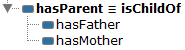
\includegraphics[width=\figwidth]{figures/new/childof_property.PNG}\caption{The property hierarchy for \con{isChildOf} and associated son/daughter properties}\label{fig:childof}
\end{center}
\end{figure}

Thus we must resort to hand assertions of properties to test out our new path:
\steps{Sons and daughters}{
\item Add the property hierarchy shown in Figure~\ref{fig:childof}, together with the equivalent property axiom and the obvious inverses.
\item As a test (after running the reasoner), ask the DL query \con{isChildOf value \ids} and you should have the answer of Richard and Robert;
\item Add the sub-property paths as described in the text;
\item Add the assertions shown in Table~\ref{tab:sibs2};
\item Run the reasoner;
\item Ask the DL query for the brother of \rds and the sister of Janet.
}

Of course, it works, but we see the same problem as above. As usual, think of the objects involved. Robert \con{isSonOf} David and David \con{isParentOf} Robert, so Robert is his own brother.{\herebedragons} Irreflexivity again causes problems as it does above (see page \pageref{pg:irreflexive}).

\begin{table}
\caption{\label{tab:sibs2}Child property assertions for the \fhkb}
\begin{tabular}{|l|l|l|}
\hline
Child & property & Parent \\
\hline
Robert David Bright 1965 & isSonOf & David Bright 1934, Margaret Grace Rever 1934 \\
Richard John Bright 1962 & isSonOf & David Bright 1934, Margaret Grace Rever 1934 \\
Mark Bright 1956 & isSonOf & John Bright 1930, Joyce Gosport \\
Ian Bright 1959 & isSonOf & John Bright 1930, Joyce Gosport \\
Janet Bright 1964 & isDaughterOf & John Bright 1930, Joyce Gosport \\
William Bright 1970 & isSonOf & John Bright 1930, Joyce Gosport \\
\hline
\end{tabular}
\end{table}

\section{Siblings: Option two}

Our option one has lots of problems. So, we have an option of asserting the various levels of sibling. We can take the same basic structure of sibling properties as before, but just fiddle around a bit and rely on more assertion while still trying to infer as much as possible. We will take the following approach:
\begin{itemize}
\item We will take off the sub-property chains of the sibling properties as they do not work;
\item We will assert the leaf properties of the sibling sub-hierarchy sparsely and attempt to infer as much as possible.
\end{itemize}

Do the following:
\steps{Add sibling assertions}{
\item Remove the sub-property chains of the sibling properties and the \con{isChildOf} assertions as explained above.
\item Add the Sibling assertions shown in table~\ref{tab:sibs};
\item Run the reasoner;
\item Ask \con{isBrotherOf value \irds};
\item Ask \con{isBrotherOf value \irjs};
\item Ask \con{hasBrother value \irds};
\item Ask \con{hasBrother value \irjs};
\item Ask \con{isSisterOf value William\_Bright\_1970};
\item Ask the query \con{Man and hasSibling value \irds}.
}

\begin{table}
\caption{\label{tab:sibs}The sibling relationships to add to the \fhkb.}
\begin{tabular}{|l|l|l|}
\hline
\bf \person &\bf Property &\bf \person \\
\hline
Robert David Bright 1965 & isBrotherOf & Richard John Bright 1962 \\
David Bright 1934 & isBrotherOf & John Bright 1930 \\
David Bright 1934 & isBrotherOf & Peter William Bright 1941 \\
Janet Bright 1964 & isSisterOf & Mark Bright 1956 \\
Janet Bright 1964 & isSisterOf & Ian Bright 1959 \\
Janet Bright 1964 & isSisterOf & William Bright 1970 \\
Mark Bright 1956 & isBrotherOf & Ian Bright 1959 \\
Mark Bright 1956 & isBrotherOf & Janet Bright 1964 \\
Mark Bright 1956 & isBrotherOf & William Bright 1970 \\
\hline
\end{tabular}
\end{table}

We can see some problems with this option as well:
\begin{itemize}
\item With these properties asserted, Richard only has a \con{hasBrother} property to Robert. We would really like an \con{isBrotherOf} to Robert to hold.
\item The query \con{Man and hasSibling value Robert} only retrieves Robert himself. Because we only asserted that Robert is a brother of Richard, and the domain of \con{isBrotherOf} is \con{Man} we know that Robert is a \con{Man}, but we do not know anything about the \con{Sex} of Richard.
\end{itemize}

\subsection{Which Modelling Option to Choose for Siblings?}

Which of the two options gives the worse answers and which is the least effort? Option~one is obviously the least effort; we only have to assert the same parentage facts as we already have; then the sub-property chains do the rest. It works OK for \con{hasSibling}, but we cannot do brothers and sisters adequately; we need \man \con{and hasSibling} $\sqsupset$ \con{isBrotherOf} and we cannot do that implication. This means we cannot ask the questions we need to ask.\herebedragons

So, we do option~two, even though it is hard work and is still not perfect for query answering, even though we have gone for a sparse assertion mode. Doing full sibling assertion would work, but is a lot of effort.

We could start again and use the \con{isSonOf} and \con{isDaughterOf} option, with the sub-property chains described above. This still has the problem of everyone being their own sibling. It can get the sex specific sibling relationships, but requires a wholesale re-assertion of parentage facts. We will continue with option~two, largely because it highlights some nice problems later on.

\section{Half-Siblings}
In Section~\ref{sec:sib1} we briefly talked about half-siblings. So far, we have assumed full-siblings (or, rather, just talked about siblings and made no distinction). Ideally, we would like to accommodate distinctions between full- and half-siblings; here we use half-siblings, where only one parent is in common between two individuals, as the example. The short-answer is, unfortunately, that \owlii cannot deal with half-siblings in the way that we want - that is, such that we can infer properties between named individuals indicating full- or half-sibling relationships.

It is possible to find sets of half-brothers in the \fhkb by writing a defined class or DL-query for a particular individual.{\herebedragons\} The following fragment of OWL defines a class that looks for the half-brothers of an individual called `Percival':
\\
\\
\owlcode{Class: HalfBrotherOfPercival

    EquivalentTo: 
        Man
         and (((hasFather some (not (isFatherOf value Percival)))
         and (hasMother some (isMotherOf value Percival)))
         or ((hasFather some (isFatherOf value Percival))
         and (hasMother some (not (isMotherOf value Percival)))))
}
\\
Here we are asking for any man that either has Percival's father but not his mother, or his mother, but not his father. This works fine, but is obviously not a  general solution. The OWL description is quite complex and the writing will not scale as the number of options (hypothetically, as the number of parents increases\ldots) increases; it is fine for man/woman, but go any higher and it will become very tedious to write all the combinations.

Another way of doing this half-brother class to find the set of half-brothers of a individual is to use cardinality constraints:
\\
\\
\owlcode{
Class: HalfBrotherOfPercival

    EquivalentTo: 
        Man
         and (hasParent exactly 1 (isParentOf value Percival))
}
\\

This is more succinct. We are asking for a man that has exactly one parent from the class of individuals that are the class of Percival's parents. This works, but one more constraint has to be present in the \fhkb. We need to make sure that there can be only two parents (or indeed, just a specified number of parents for a person). If we leave it open as to the number of parents a person has, the reasoner cannot work out that there is a man that shares exactly one parent, as there may be other parents. We added this constraint to the \fhkb in Section~\ref{sec:nom_owa}; try out the classes to check that they work.

These two solutions have been about finding sets of half-brothers for an individual. What we really want in the \fhkb is to find half-brothers between any given pair of individuals.
% Figure~\ref{fig:half-sibs} shows some example person individuals with parentage relationships between them; the diagram shows two full-siblings and one half-sibling. We will use this diagram to help us work through how \owlii and a reasoner would have to work out sibling relationships. First of all, this task is easily achieved with an SPARQL query or a DL-safe~\cite{dl-safe} rule. 
%The rule to find full-siblings would look something like
%\\
%\\
%\owlcode{
%hasParent(A,Y) and hasParent(A,X) and 
%Y not equals X and 
%hasParent(C,X) and hasParent(C,Y) and 
%A not equals C 
%}\\
%That is, A and C are full-siblings if A and C are different, the X and Y parents are shared by both A and C and are distinct individuals. A similar rule can be constructed for half-siblings:
%\\
%\\
%\owlcode{
%hasParent(A,Y) and hasParent(A,X) and 
%Y not equals X not = z and 
%hasParent(C,X) and hasParent(C,z) and 
%A not equals C 
%}\\
%That is, A and C are half-siblings if A and C are different, the X, Y and Z parents are shared by both A and C and are distinct individuals. 

%\begin{figure}
%\begin{center}
%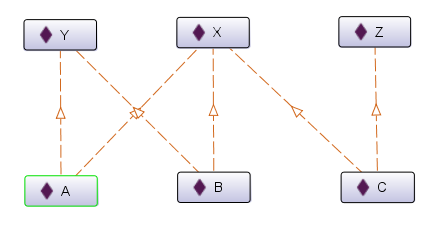
\includegraphics[width=\figwidth]{figures/new/halfsiblings}
%\caption{A, B and C are the child generation, X, Y and Z are the parent generation. Using the \con{hasParent} with \con{isParentOf} as a route between child, a parent and another child, we can see A and B are full-siblings as their two parents are the same. C is a half-sibling of the other two, as C only has one parent in common. We are assuming all individuals are different.}
%\label{fig:half-sibs}
%\end{center}
%\end{figure}

%These rules work OK, but we want to use OWL plus an automated reasoner to give the relationships between two named individuals. However, doing this just in \owlii is not possible. Look at the individuals in Figure~\ref{fig:half-sibs} and trace what a sub-property chain would have to do (bear the rules above in mind too, it can help):

%\begin{enumerate}
%\item We have a sub-property chain \con{hasParent o isParentOf}. This goes from a person to another person via the parentage relationships.
%\item Looking at Figure~\ref{fig:half-sibs}, we can see that to find full-siblings, one traces the path twice and the parents have to number only two - there are only two routes. 
%\item If we look at individuals A and C, then we have three possible routes and we conclude that a half-sibling relationship holds between A and C.
%\item Instead of counting routes, what we're doing is looking at the number of distinct individuals that are the set of intermediate objects on the path; for full-siblings it's two and for half-siblings it's three.
%\end{enumerate}

%OWL cannot do this kind of counting. We have the parentage lines going up and down, as a tree. What we want to do is cut across this tree to check, for example, that x and y are different.
%OWL cannot cut across this tree \todo{point at some ref}. It is possible in logics other than the fragment of description logic upon which OWL is based \todo{and could be part of OWL}, but is not part of the recommendation. 
%
%We have not even tried sex yet. To get brother or sister relationships, we need to know the sex of one of the objects. This is hard and is not part of the OWL recommendation. The work described in \cite{manMan09} will help us out. We need sex in at least two places. First, we want \con{Man and hasSibling} to imply \con{isBrotherOf}; this  is known as the `man man' problem and is not part of the \owlii recommendation. Second, the same need comes up when we move outside the narrow biological view of parentage and conservative view of marriage (see Chapter~\ref{chap:marriage}) that we take in this tutorial. We write the sub-property chain in option one above as \con{hasParent o isParentOf}; if we could write a pair of sub-property chains \con{hasParent o Man o isParentOf} together with \con{hasParent o Woman o isParentOf}, then we have described biological parentage. We could account for same sex parentage if we could put sex into the intermediate objects, but may wish to distinguish adoptive parentage etc. by other means.

Unfortunately we cannot, without rules, ask \owlii to distinguish full- and half-siblings -- we cannot count the number of routes taken between siblings via different distinct intermediate parent objects. %In addition, we cannot use conjunctions between an object and a property to imply another property. These are possible in logics outside the one used in \owlii.

\section{Aunts and Uncles}

An uncle is a brother of either my mother or father. An aunt is a sister of either my mother or father. In common practice, wives and husbands of aunts and uncles are usually uncles and aunts respectively. Formally, these aunts and uncles are aunts-in-law and uncles-in-law. Whatever approach we take, we cannot fully account for aunts and uncles until we have information about marriages, which will not have until Chapter~\ref{chap:marriage}. We will, however, do the first part now.

Look at the objects and properties between them for the following facts:
\begin{itemize}
\item Robert has father David and mother Margaret;
\item David has brothers Peter and John;
\item Margaret has a sister Eileen;
\item Robert thus has the uncles John and Peter and an aunt Eileen.
\end{itemize}

As we are tracing paths or `chains' of objects and properties we should use sub-property chains as a solution for the aunts and uncles. We can make an \con{hasUncle} property as follows (see Figure~\ref{fig:uncle_path}):
\\\\
\owlcode{
ObjectProperty: hasUncle

SubPropertyOf: hasBloodrelation

Domain: Person

Range: Man

SubPropertyChain: hasParent o hasBrother

InverseOf: isUncleOf
}
\\
\begin{figure}
\begin{center}
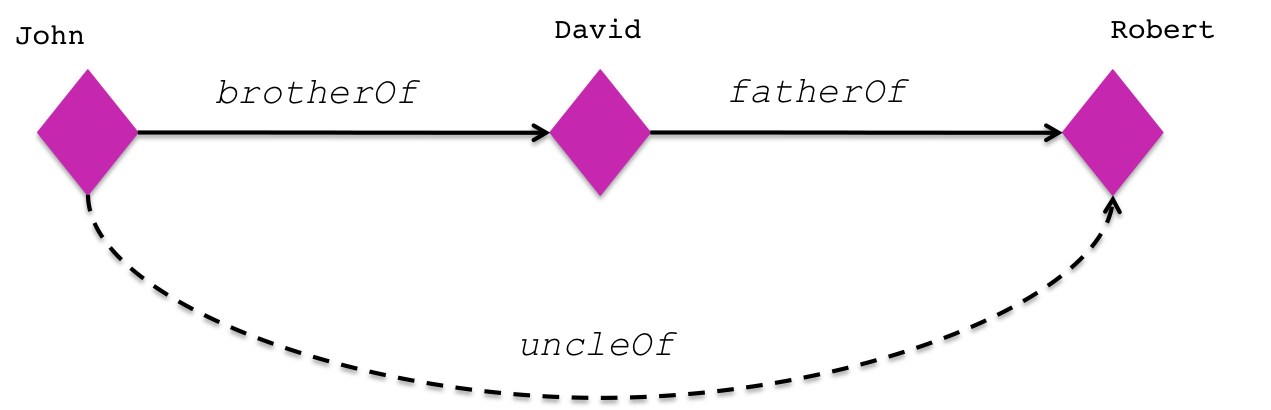
\includegraphics[width=\figwidth]{figures/uncle}\caption{Tracing out the path between objects to get the \con{hasUncle} sub-property chain.}\label{fig:uncle_path}
\end{center}
\end{figure}

Notice we have the domain of \man and range of \person. We also have an inverse. As usual, we can read this as `an object that holds an \con{hasParent} property, followed by an object holding a \con{hasBrother} property, implies that the first object holds an \con{hasUncle} property with the last object'.

Note also where the properties (include the ones for aunt) go in the object property hierarchy. Aunts and uncles are not ancestors that are in the direct blood line of a person, but they are blood relations (in the narrower definition that we are using). Thus the aunt and uncle properties go under the \con{hasBloodrelation} property (see Figure~\ref{fig:uncleprops}). Again, think of the implications between objects holding a property between them; that two objects linked by a property implies that those two objects also hold all the property's super-properties as well. As long as all the super-properties are true, the place in the object property hierarchy is correct (think about the implications going up, rather than down).

\begin{figure}
\begin{center}
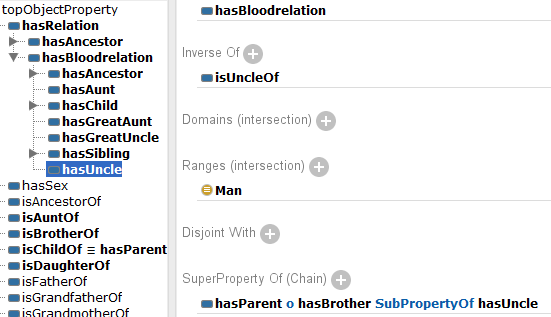
\includegraphics[width=\textwidth]{figures/new/prop_uncle.PNG}
\caption{The object property hierarchy with the aunt and uncle properties included. On the right side, we can see the hasUncle property as shown by \protege.}\label{fig:uncleprops}
\end{center}
\end{figure}
 
Do the following tasks:
\steps{Uncles and Aunts}{
\item Add the \con{hasUncle} property as above;
\item Add the \con{hasAunt} property as well;
\item Ask for the uncles of \con{Julie\_Bright\_1966} and for \con{Mark\_Bright\_1956};
\item Add similar properties for \con{hasGreatUncle} and \con{hasGreatAunt} and place them in the property hierarchy.
}

We can see this works -- unless we have any gaps in the sibling relationships (you may have to fix these). Great aunts and uncles are simply a matter of adding another `parent' leg into the sub-property chain. We are not really learning anything new with aunts and uncles, except that we keep gaining a lot for free through sub-property chains. We just add a new property with its sub-property chain and we get a whole lot more inferences on individuals. To see what we now know about \rds, do the following:

\steps{What do we know?}{
\item Save the ontology and run the reasoner; 
\item Look at inferences related to the individual \rds (see warning in the beginning of this chapter).
\item If you chose to use DL queries in \protege, do not forget to tick the appropriate checkboxes.
}

You can now see lots of facts about \rds, with only a very few actual assertions directly on \rds.

\section{Summary}

Siblings have revealed several things for us:
\begin{itemize}
\item We can use just the parentage facts to find siblings, but everyone ends up being their own sibling;
\item We cannot make the properties irreflexive, as the knowledge base becomes inconsistent;
\item We would like an implication of \man and \con{hasSibling} $\supset$ \con{isBrotherOf}, but \owlii doesn't do this implication;
\item Whatever way we model siblings, we end up with a bit of a mess;
\item \owlii cannot do half-siblings;
\item However, we can get close enough and we can start inferring lots of facts via sub-property chains using the sibling relationships.
\end{itemize}

\expressivity{SRIF}

\ctime{1355614}{206}{39}